\section{System with sequential composition}
    We model a first system with two sequentially composed components. We choose to model the two components as M/M/1/K queues. \\
    This is because an average component in a distributed system can be modeled as an M/M/1/K queue. This is due to the exponential inter-arrival rate of messages, the exponential distribution of the execution delays, the buffer size of messages $K$ of a component and its failure rate $f$. \cite{dq-tut}
    
    Let us first provide a refresher about M/M/1/K queues:
    \begin{itemize}
        \item $\lambda$: The arrival rate.
        \item The service time $s$: is the time it takes to serve a message.
        \item $\mu$: The service \textbf{rate} and E[s] = $\frac{1}{\mu}$
        \item Offered load: $\rho = \dfrac{\lambda}{\mu}$
    \end{itemize}

    We will control $\lambda$ to show its effects on the offered load. This is because the offered load can tell much about the system:
    \begin{itemize}
        \item At low load ($\rho < 0.8$) the failure will tend to 0. The system is behaving correctly and the $\Delta$Q will show that, as the delay will tend to 1.
        \item Once $\rho$ is approaching high load ($\rho > 0.8$) we can observe the failure increasing quickly. However, we can observe the system starting to get bad after $\rho > 0.5$. \cite{dq-tut}
    \end{itemize}
    
    \subsection{System's outcome diagram}
    The system (\cref{fig:mm1k}) has two components \texttt{worker\_1}, \texttt{worker\_2}. Each individual component is composed of a queue of size $K = 1000$ and a worker process.
    
    The system sends $n$ messages per second following a Poisson distribution to \texttt{worker\_1}'s queue. 
    The queue notifies its worker if the worker is not busy. The worker performs $N$ loops of fictional work, they are defined upon start and are done to simulate a component performing a task. Once done, \texttt{worker\_1} then passes a message to \texttt{worker\_2}'s queue, which has another queue of size = 1000, who passes the message to \texttt{worker\_2}'s worker, which does the same amount of loops as \texttt{worker\_1}. When a worker completes its work, it notifies its queue, freeing one message from its buffer size and allowing the next message to be processed.
    
    If the queue's buffer is overloaded, it will drop the incoming message and consider the execution a failure.
    
    A probe named ``$probe$'' is defined, which observes the execution from when the message is sent to \texttt{worker\_1} up until \texttt{worker\_2} is done.

    Lastly, both workers share the same processor, to observe the effects of non-linearity in a distributed setting.

    The system can be defined via the previously defined syntax (\cref{out_syntax}) as: 
    
    \begin{minted}{text}
        probe = worker_1 -> worker_2;
    \end{minted}

    \begin{figure}[H]
        \begin{center}
            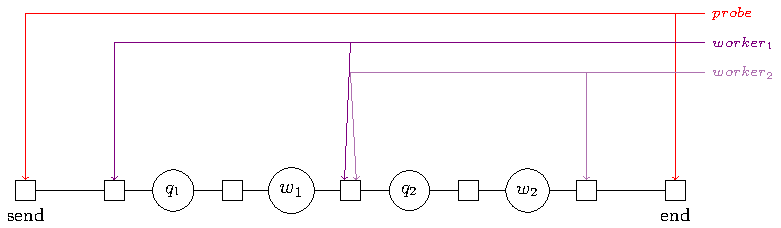
\includegraphics[scale=1]{tikz/mm1k.pdf} 
        \end{center}
        \caption{Refined outcome diagram of the system. The labeled coloured lines represent the probes that were inserted. $q_{1, 2}$ outcomes represent the queues. $w_{1,2}$ represent the workers. As we do not wish to observe the queues, but the whole behaviour of the worker components, we can insert probes from when the message is received to when the worker loops end. We can imagine that $q_{1,2}$ and $w_{1,2}$ are refinements of outcomes $worker_{1,2}$, this is why the probes names differ from the outcomes they observe.}
        \label{fig:mm1k}
    \end{figure}

    \subsection{Determining parameters dynamically}
        We stated previously that determining parameters is something that must be done with an underlying knowledge of the system (\cref{subsec:dMax}). The oscilloscope can provide knowledge of the system. \cref{fig:w1w2hb} shows an example of worker\_1 and worker\_2 as observed in the oscilloscope.

        The engineer supposes that the workers executions should take a maximum of 4 ms to complete, but doesn't actually know how long the executions should take. The engineer, after having set $dMax = 4ms$, observes the graph \cref{fig:w1w2hb} on the left in the oscilloscope.

    The oscilloscope shows the engineer that their assumptions do not correspond to the actual system $\Delta$Q. The user can then modify the parameters to observe the actual worker's behaviour. By setting $dMax$ to 8 ms, they can observe the worker's $\Delta$Qs failure approaching $0$ on the right Figure in \cref{fig:w1w2hb}.

    On the other hand, the engineer's assumption could have been what they truly expected from the system. In this case, the oscilloscope tells him that the system is not behaving as expected. 

\begin{figure}[H]
            \centering
            \begin{subfigure}{.5\textwidth}
                \centering
                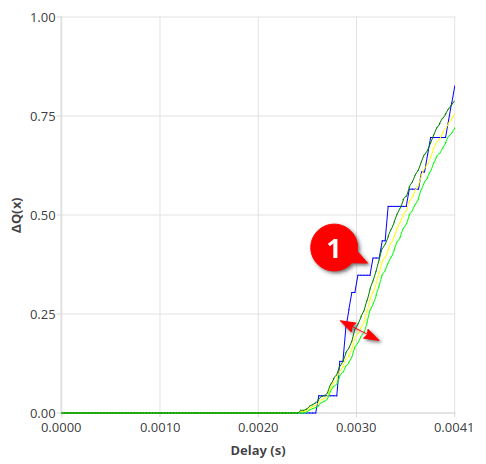
\includegraphics[width=0.98\textwidth]{img/overload_2/worker_1a.png}
                \label{fig:w14}
            \end{subfigure}%
            \begin{subfigure}{.5\textwidth}
                \centering
                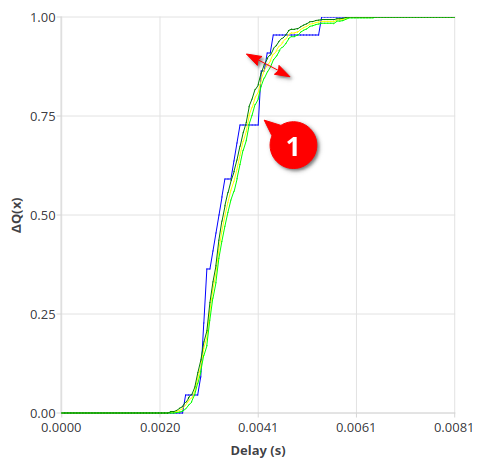
\includegraphics[width =0.98\textwidth]{img/overload_2/worker_1_8a.png}
                \label{fig:w18}
            \end{subfigure}
            \caption{\textbf{Left}: worker\_1 $\Delta$Q with $dMax = 4ms$. (Green, between the arrow): Mean and confidence bounds of $\Delta$Qs in polling window. (1, blue): Observed $\Delta$Q in sampling window. The worker failure tends to 0.25. \\
            \textbf{Right}: worker\_1 $\Delta$Q with $dMax$ = 8ms. The worker failure now tends to 0. \\
            In both graphs we can observe how the observed $\Delta$Q of the sampling window is not precise. The step function representation of it fluctuates. The mean and confidence bounds provide a more precise representation of the $\Delta$Qs of worker\_1 over a polling window.}%
            \label{fig:w1w2hb}
            \end{figure}

    \subsubsection{Low Load} 
   We will send 50 messages per second to observe the system under test to get key properties. The workers do a million loops. \\
    We can observe in the left graph in \cref{fig:norm_ex} that the average worker's execution takes $\approx$ 33ms. We then have $\mu_{worker} = \frac{1}{0.0033 s} \approx 300$ req/s. Thus, $\rho = \frac{50}{300} = 0.1\overline{6}$, we can assume the system is at low load.

    At low load (\cref{fig:norm_ex}), the system is behaving \textbf{linearly}. Recall \cref{indep_hyp}, at low load the sum of the two delays will overlap with the observed total delay. We can observe in the oscilloscope the probe \textbf{observed $\Delta$Q} and \textbf{calculated $\Delta$Q} confidence bounds overlap. 
        \begin{figure}[H]
            \centering
            \begin{subfigure}{.5\textwidth}
                \centering
                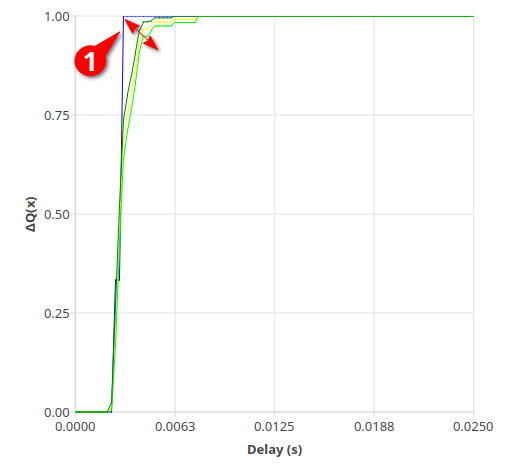
\includegraphics[width=0.98\textwidth]{img/overload_2/50_workeran.png}
                \label{fig:norm_ex_1}
            \end{subfigure}%
            \begin{subfigure}{.5\textwidth}
                \centering
                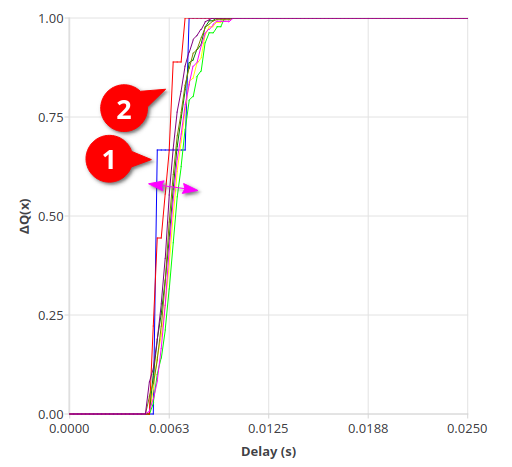
\includegraphics[width =0.98\textwidth]{img/overload_2/50_probe2.png}
                \label{fig:norm_ex_2}
            \end{subfigure}
            \caption{Graphs for $\lambda = 50$. Left: worker\_1 $\Delta$Qs. (1, Blue): The observed $\Delta$Q. (Green, between arrows): Observed polling window confidence bounds. \\
            Right: ``probe'' $\Delta$Qs. (1, blue): The sampling window observed $\Delta$Q. (2, red): The sampling window calculated $\Delta$Q. (Magenta, between arrows): the observed and calculated $\Delta$Qs confidence bounds overlapping.}
            \label{fig:norm_ex}
        \end{figure}
    
\subsubsection{Early signs of overload}
    
    At load = 0.5 the system should start showing dependent behaviour. We can observe what happens when $\lambda = 150 \rightarrow \rho = 0.5$.
    
    Recall \ref{fig:cdf_indep}, a non-linear system does not obey superposition. The sum of the delay of the workers will deviate from the overall delay of ``probe''. In \cref{fig:ovovv}, this is the case. \\
    We can start to observe early signs of dependency even at $\rho = 0.5$. The mean of the observed $\Delta$Q is deviating from the calculated one. At the 50th percentile the deviation is \textit{minimal}, around 0.4 ms. Nevertheless, the precision of the paradigm and the oscilloscope allows even for these minimal deviations to appear on the graphs, being able to recognise \textit{non-linearity} and \textit{early signs of overload}. \\
    The superposition principle is not respected anymore, there is apparent \textbf{non-linearity}, and the fact that $\Delta$Q can recognise non-linear behaviour with \textbf{0.4ms precision} is impressive. The oscilloscope is a powerful tool that can help assess dependent behaviour in running systems.
 
       \begin{figure}[H]
            \centering
            \begin{subfigure}{.5\textwidth}
                \centering
                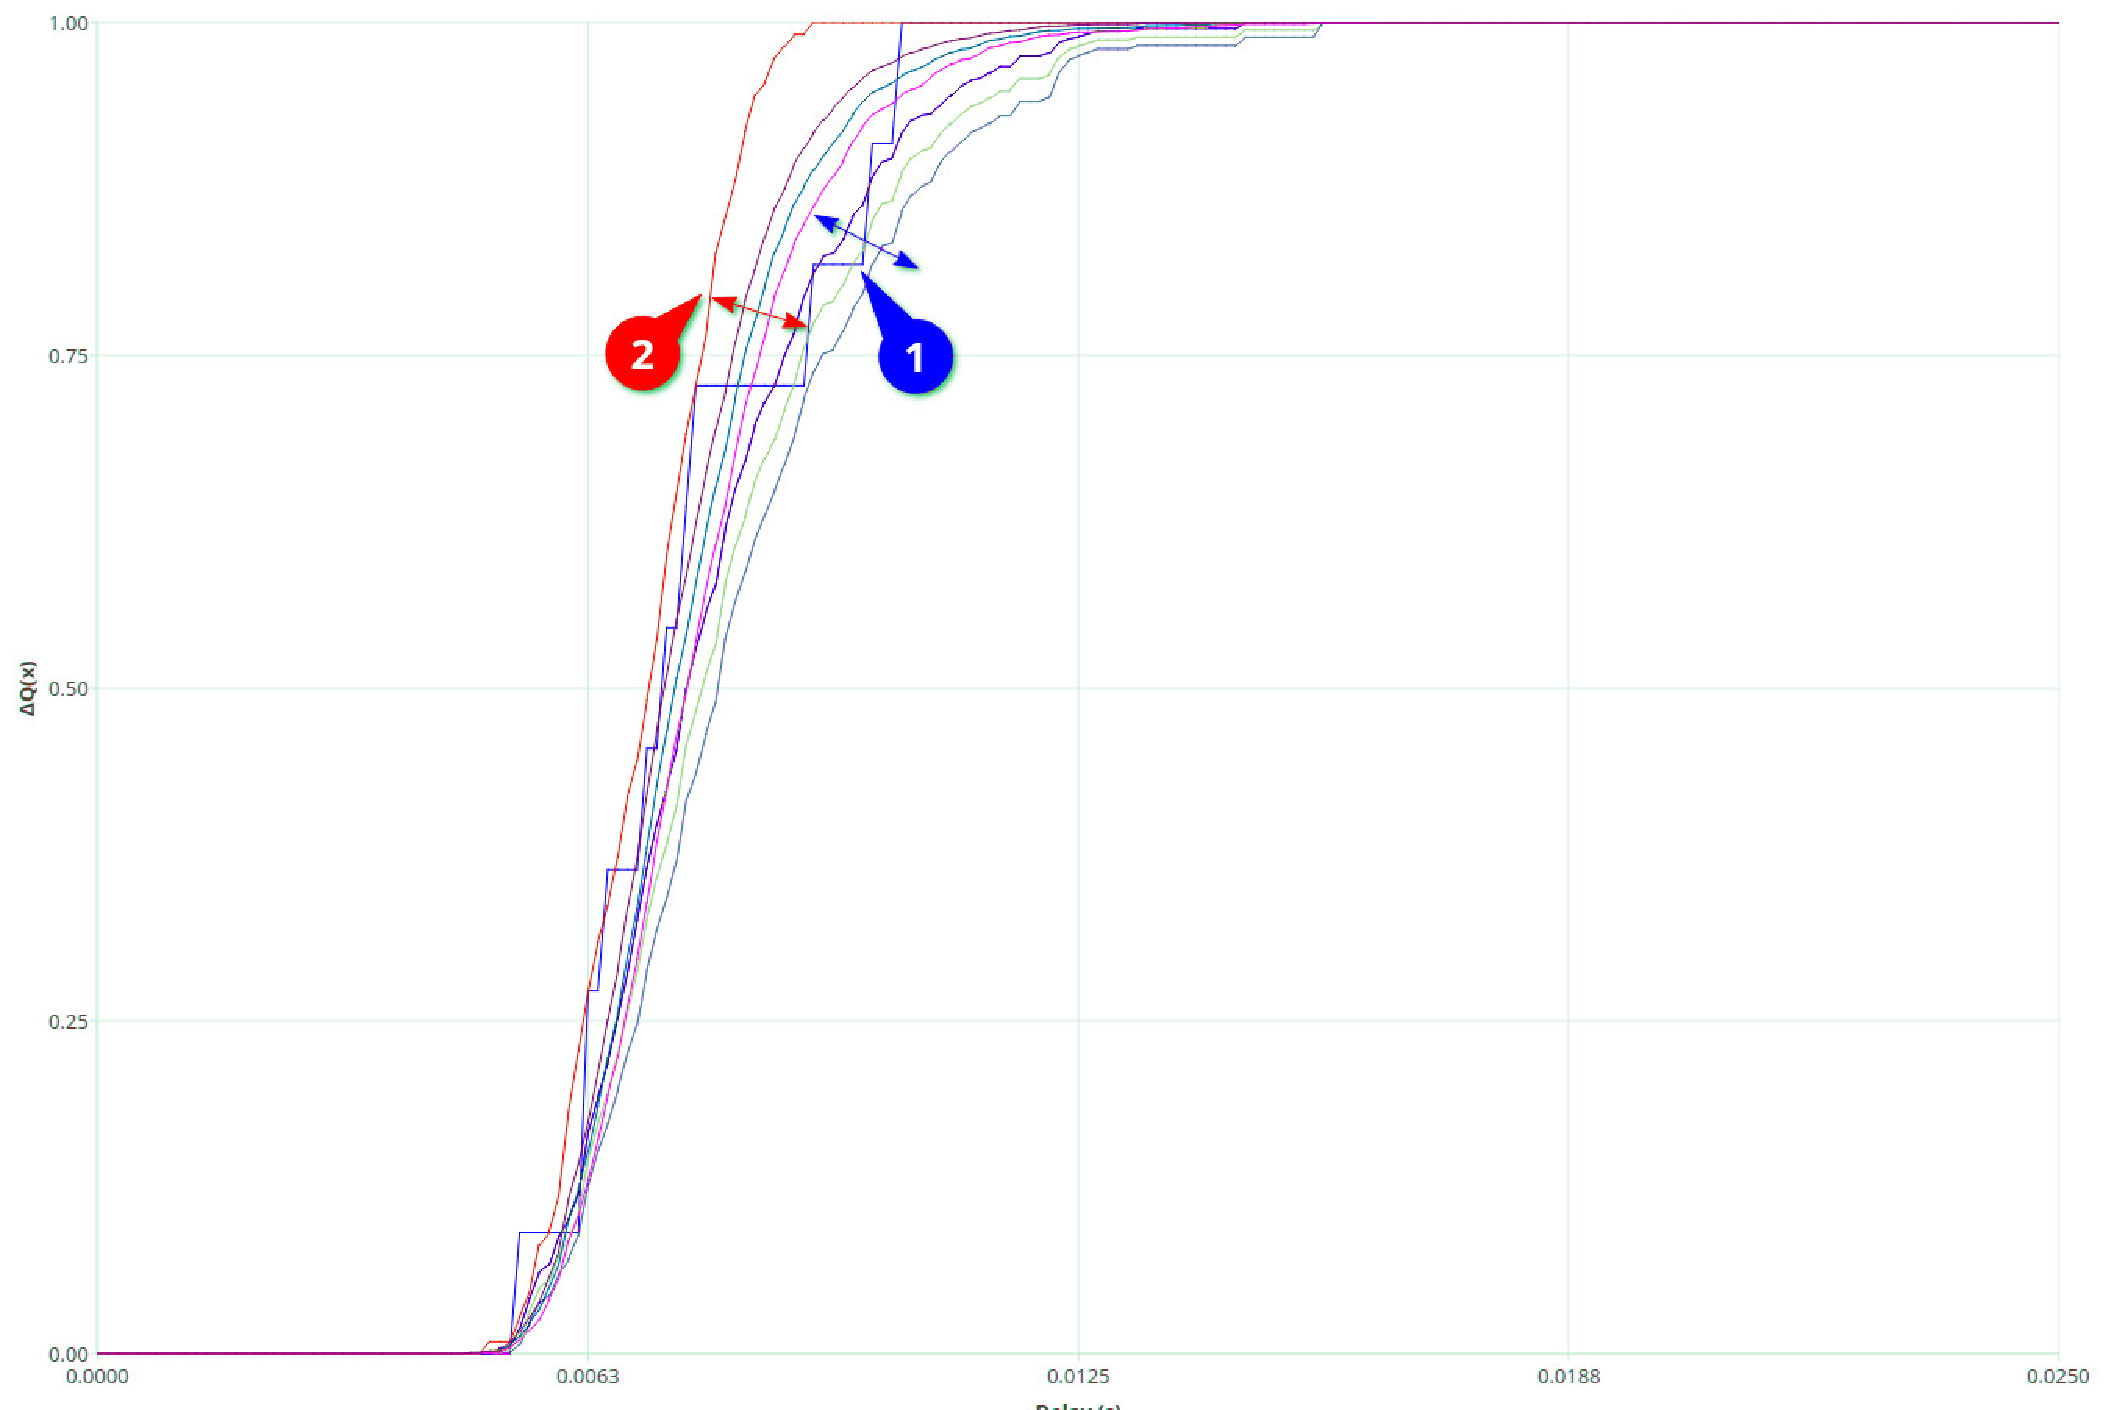
\includegraphics[width=0.98\textwidth]{img/overload_2/150_probe2.pdf}
                \label{fig:ovuvv}
            \end{subfigure}%
            \begin{subfigure}{.5\textwidth}
                \centering
                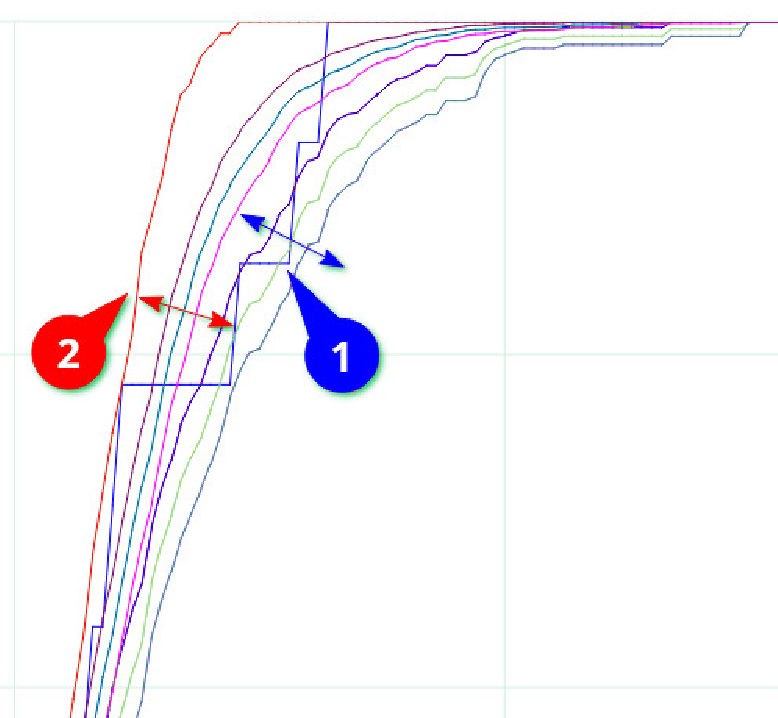
\includegraphics[width =0.98\textwidth]{img/overload_2/150_probe2zoom_cropped.pdf}
                \label{fig:ovovv}
            \end{subfigure}
            \caption{\textbf{Left}: The ``probe'' $\Delta$Qs as observed in a snapshot. \textbf{Right}: Zooming in the oscilloscope, we can observe a slight, but noticeable deviation. (1) Sampling window observed $\Delta$Q. (Arrow, blue, above): Its confidence bounds. (2) Sampling window calculated $\Delta$Q. (Arrow, red, below): Its confidence bounds. \\ The observed polling window confidence bounds are $>$ than the calculated $\Delta$Q bounds. The deviation at the median is of 0.4 ms, but it is noticeable in the oscilloscope.}
            \label{fig:avavv} 
        \end{figure}
       
\subsubsection{High load}
    Performance degradation at 0.5 offered load is already remarkable, the observed $\Delta$Qs and the calculated ones are slowly but surely deviating. The difference is seemingly minimal, but noticeable. We can go even further and observe the system under high load situations (\cref{fig:early_ov}). We set $\lambda = 250 \rightarrow \rho = 0.83$, just above the high load threshold.
    
       \begin{figure}[H]
            \centering
            \begin{subfigure}{.5\textwidth}
                \centering
                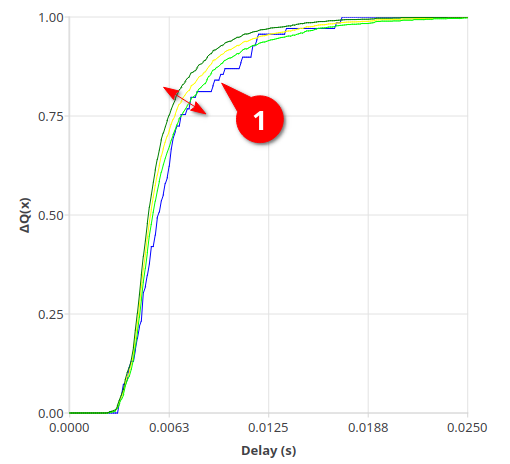
\includegraphics[width=0.98\textwidth]{img/overload_2/250_workera.png}
                \label{fig:high_load_1}
            \end{subfigure}%
            \begin{subfigure}{.5\textwidth}
                \centering
                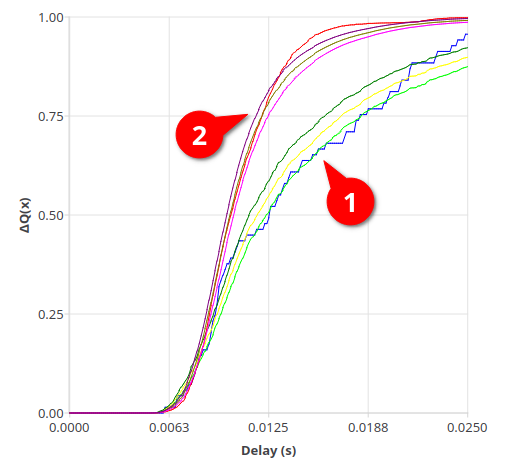
\includegraphics[width =0.98\textwidth]{img/overload_2/250_probe2.png}
                \label{fig:high_load_2}
            \end{subfigure}
            \caption{Graphs for $\lambda = 250$. \textbf{Left}: worker\_1 observed $\Delta$Q with its confidence bounds. \\
            \textbf{Right}: probe $\Delta$Qs. (1, blue) Sampling window observed $\Delta$Q with its confidence bounds, (2, red) Sampling window calculated $\Delta$Q inside its confidence bounds.}%
            \label{fig:early_ov}
        \end{figure} 
    This confirms what is expected by queueing theory, $\Delta$Q is capable of observing the basic observation requirements and capable of recognising dependency. While what is expected by the worker's observed $\Delta$Q is a nice normally distributed CDF with little to no failure. What we can observe on the probe is degraded performance in its observed $\Delta$Q mean. \\
    Due to dependency, high load and processor utilisation, the queue is filling up and the workers are taking more time to complete. If you recall \cref{fig:norm_ex}, the worker's delay distribution was less than the current one. We can see that it has completely degraded, with the average request taking almost double the time as under normal queueing conditions. 

    Further degradation can be observed by increasing $\lambda = {300, 350} \rightarrow \rho \ge 1$ (\cref{fig:hi_lo}).

    \begin{figure}[H]
            \centering
            \begin{subfigure}{.5\textwidth}
                \centering
                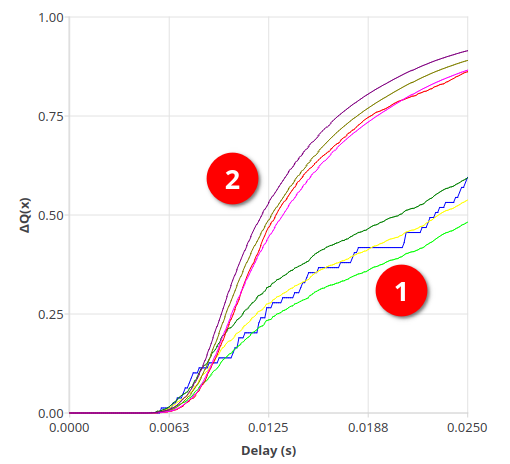
\includegraphics[width=0.98\textwidth]{img/overload_2/300_probe2.png}
                \label{fig:high_load_1}
            \end{subfigure}%
            \begin{subfigure}{.5\textwidth}
                \centering
                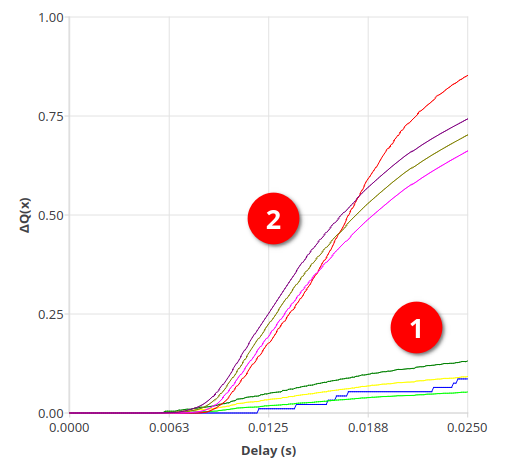
\includegraphics[width =0.98\textwidth]{img/overload_2/350_probe2.png}
                \label{fig:high_load_2}
            \end{subfigure}
            \caption{\textbf{Left}: (1) probe observed $\Delta$Q and confidence bounds for polling window. (2) probe calculated $\Delta$Q and confidence bounds for polling window at $\lambda = 300$. \textbf{Right}: probe $\Delta$Qs at $\lambda = 350$.}%
            \label{fig:hi_lo}%
        \end{figure}
    The system degrading is clear, the $\Delta$Qs show how almost all messages are being dropped or take $> dMax$. We can now look at triggers and how they can be useful to diagnose such cases.
  
    \subsubsection{Triggers}
        By observing the system under test in high load cases, we can set the load trigger by setting the sampling window to 1 second and trigger when outcome instances $\gtrapprox 150$. We can also set a trigger based on observation of the running system.

        \paragraph{QTA trigger}
            Recall the previous definition of $\Delta$Q (\cref{subsec:qta_i}), by observing the system, we create a QTA for the probe ``probe'' with: 25\% = 0.0075 s, 50\% = 0.0125 s, 75\% = 0.015s and minimum success rate = 0.9.

            By setting the trigger to fire for $\Delta$Q$_{obs} < QTA$. We captured a handful of snapshots. Here, $\lambda = 150$.
        
        \begin{figure}[H]
            \centering
            \begin{subfigure}{.5\textwidth}
                \centering
                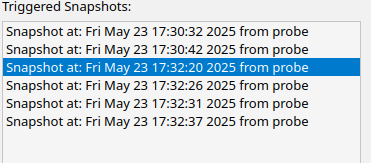
\includegraphics[width=0.98\textwidth]{img/violated.png}
                \label{fig:high_load_1}
            \end{subfigure}%
            \begin{subfigure}{.5\textwidth}
                \centering
                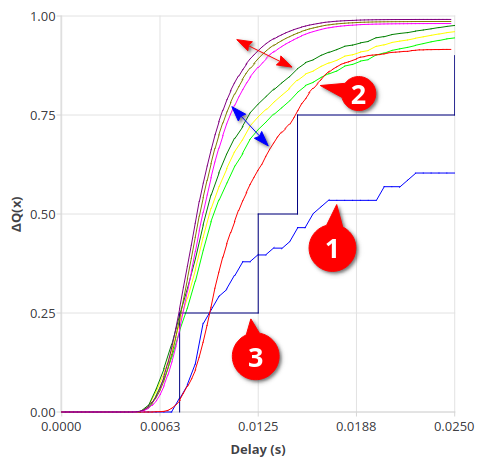
\includegraphics[width =0.98\textwidth]{img/overload_2/qta_triggerd2.png}
                \label{fig:high_load_2}
            \end{subfigure}
            \caption{\textbf{Left}: Snapshots for fired triggers. \\
            \textbf{Right}: (1, blue) Observed $\Delta$Q in sampling window violating QTA (3). The confidence bounds for the observed polling window (blue, arrow, below) show the system deteriorating. The sampling window calculated $\Delta$Q (2) is behaving worse than its confidence bounds (red, arrow, above). The system is overloaded, degrading and showing non-linear behaviour, this is captured by the QTA violation.} % 
            \label{fig:qta_viol_1}
        \end{figure}
        \paragraph{Instances trigger}

        QTA triggers can help detect non-linearity even before it becomes evident. \\
        By knowing the inner details of the system, setting a QTA on the number of instances can be useful. \cref{fig:qta_trig} is an example of a fired trigger on the number of instances. Even though the QTA requirement isn't being violated, the number of instances fires a trigger, where the user can observe that the system is showing early signs of overload.

        \begin{figure}[H]
            \begin{center}
                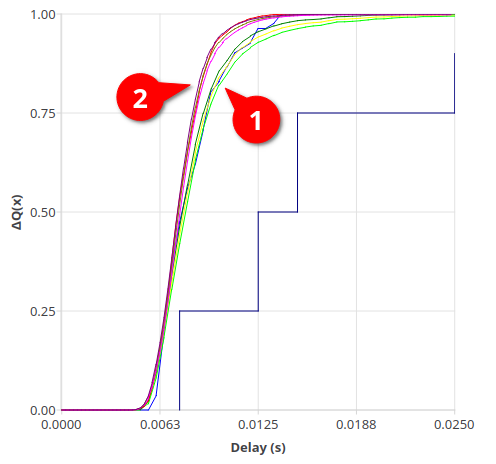
\includegraphics[scale=0.5]{img/overload_2/fired_samplea.png}
            \end{center}
            \caption{Graph of a snapshot for a fired trigger observing the load of a probe. (1) Observed $\Delta$Q confidence bounds. (2) Calculated $\Delta$Q confidence bounds. The trigger fires for observed load $> 150$ in a sampling window of 1 second. Even if the QTA requirement (step function) is not being violated, the system is showing early signs of non-linear behaviour.}%
            \label{fig:qta_trig}%
        \end{figure}
  
